\documentclass{beamer}
%Для защит онлайн лучше использовать разрешение 16x9
%\documentclass[aspectratio=169]{beamer}

\input{preamble.tex}

% То, что в квадратных скобках, отображается внизу по центру каждого слайда. 
\title[SPLA, GraphBLAS+LAGraph]{Сравнение производительности алгоритмов на графах из SPLA/GraphBLAS+LAGraph}

% То, что в квадратных скобках, отображается в левом нижнем углу. 
\institute[СПбГУ]{}

% То, что в квадратных скобках, отображается в левом нижнем углу.
\author[Гавриленко Михаил]{Гавриленко Михаил, группа 23.Б15-мм}
 
\begin{document}
{
\setbeamertemplate{footline}{}
% Лого университета или организации, отображается в шапке титульного листа
\begin{frame}
  
\includegraphics[width=1.4cm]{pictures/SPbGU_Logo.png}
\vspace{-35pt}
\hspace{-10pt}
\begin{center}
   \begin{tabular}{c}
        \scriptsize{Санкт-Петербургский государственный университет} \\
        \scriptsize{Кафедра системного программирования}
    \end{tabular}
\titlepage
\end{center}

\btVFill

\begin{center}
  \vspace{5pt}
  \scriptsize{Санкт-Петербург\\
                 2023}
  \end{center}

\end{frame}
}

\begin{frame}
  \frametitle{Постановка задачи}
  \textbf{Целью} является исследование алгоритмов BFS, SSSP, TC, PR из библиотек SPLA и GraphBLAS/LAGraph  

  \textbf{Задачи}:
  \begin{itemize}
	\item Сформулировать набор гипотез о производительности алгоритмов на основе базовых представлений о наивном алгоритме и особенностях платформ
    \item Произвести замеры производительности реализаций из выбранных библиотек
    \item Исследовать результаты и выявить особенности, отразившиеся на производительности 
	\item Сделать выводы о ранее сформулированных гипотезах 
  \end{itemize}
\end{frame}
            
\begin{frame}  
  \frametitle{Детали экспериментов}
  Использованные метрики:
  \begin{itemize}
	  \item Время выполнения (мс) 
	  \item Степень прироста производительности SPLA относительно LAGraph 
	  \item GTEPS(Giga Traversed Edges Per Second)
  \end{itemize}


  Конфигурация системы:
  \begin{itemize}
	  \item M2 Max (arm64), 38-gpu ядер 1000Мгц, 12-cpu ядер (8+4), 32ГБ ОЗУ
	  \item OpenCL 1.2
	\item clang 17.0.0
  \end{itemize}

    
\end{frame}

\begin{frame}
	\frametitle{BFS: (первичные тезисы)}
  \begin{itemize}
    \item Исполнение алгоритма эффективнее на GPU 
    \item GPU лучше справляется с симметричными датасетами, в отличии от CPU    
	\item Преобразование в неориентированный граф увеличит вычислительную нагрузку, но улучшит показатель GTEPS за счет более эффективной работы Pull-фазы (bottom-up BFS)
	\item Первая итерация на GPU будет значительно медленнее последующих из-за JIT-компиляции ядер OpenCL
  \end{itemize}
\end{frame}

\begin{frame}
	\frametitle{BFS: (детали алгоритмов)}
  Оба алгоритма являются "pull-push", однако некоторые детали различаются: 
  \begin{itemize}
	  \item SPLA выбирает push/pull по плотности текущей фронтирной структуры
	  \item LAGraph опирается на кэшированные свойства, в ином случае переключается на push-only
	  \item В SPLA есть явный early-exit 
  \end{itemize}
\end{frame}

\begin{frame}
  \frametitle{BFS}
	\centering
  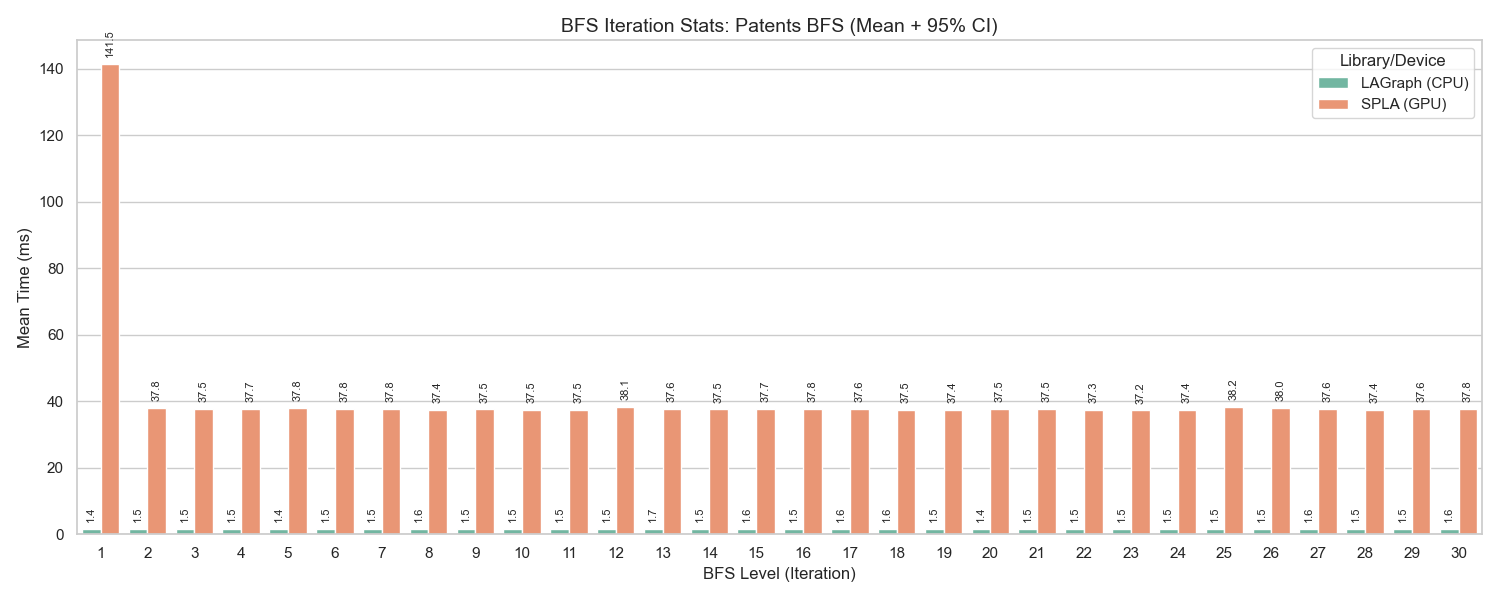
\includegraphics[width=1\textwidth]{pictures/bfs/all.png}
\end{frame}

\begin{frame}
  \frametitle{BFS}
	\centering
  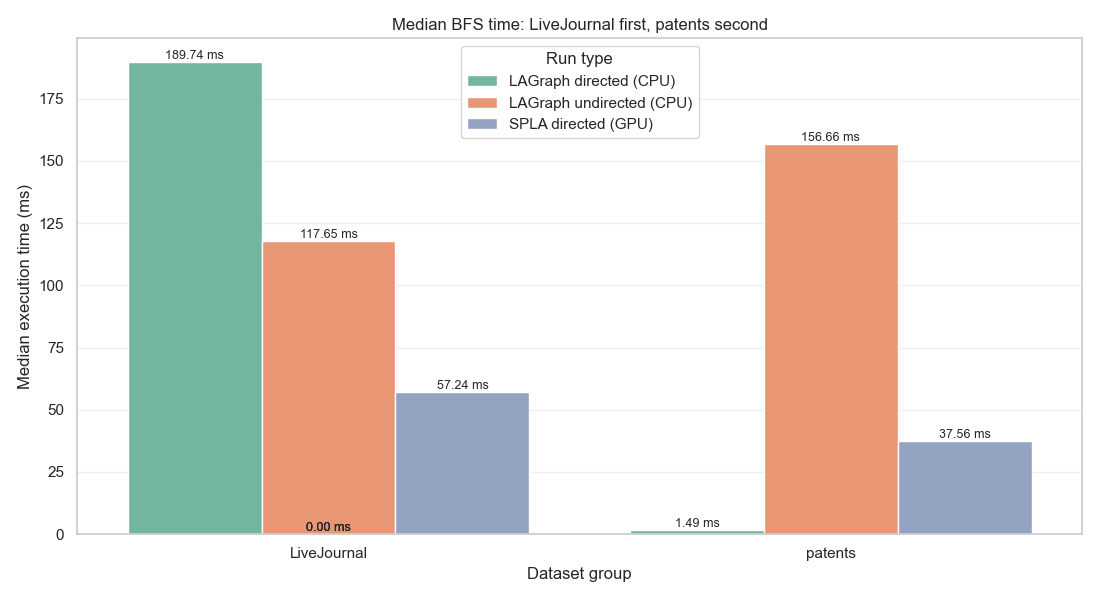
\includegraphics[width=1\textwidth]{pictures/bfs/all_mean_time.png}
\end{frame}

\begin{frame}
  \frametitle{BFS}

	\centering
  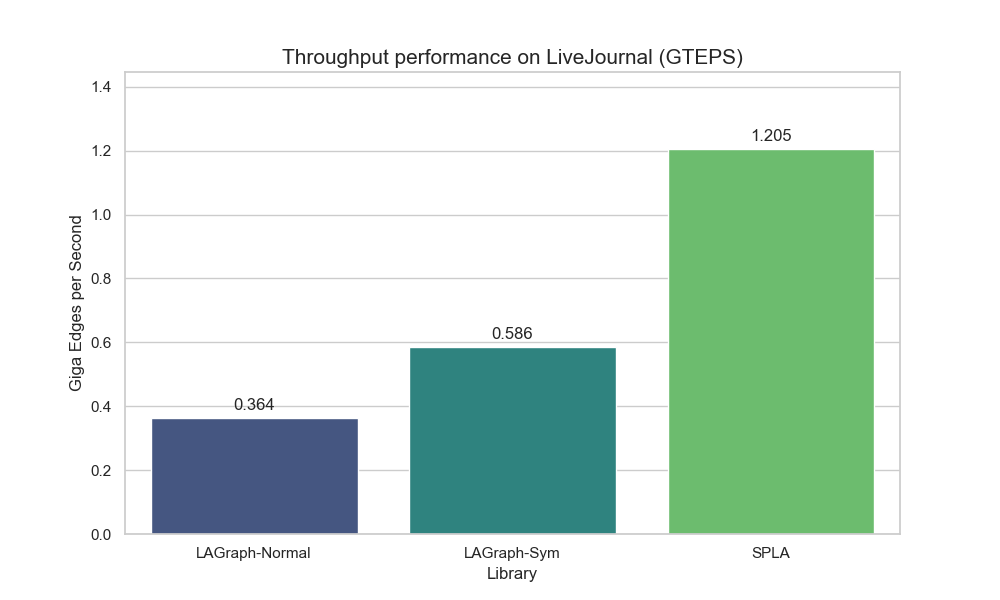
\includegraphics[width=1\textwidth]{pictures/bfs/all_gteps.png}
\end{frame}

\begin{frame}
  \frametitle{BFS}

	\centering
  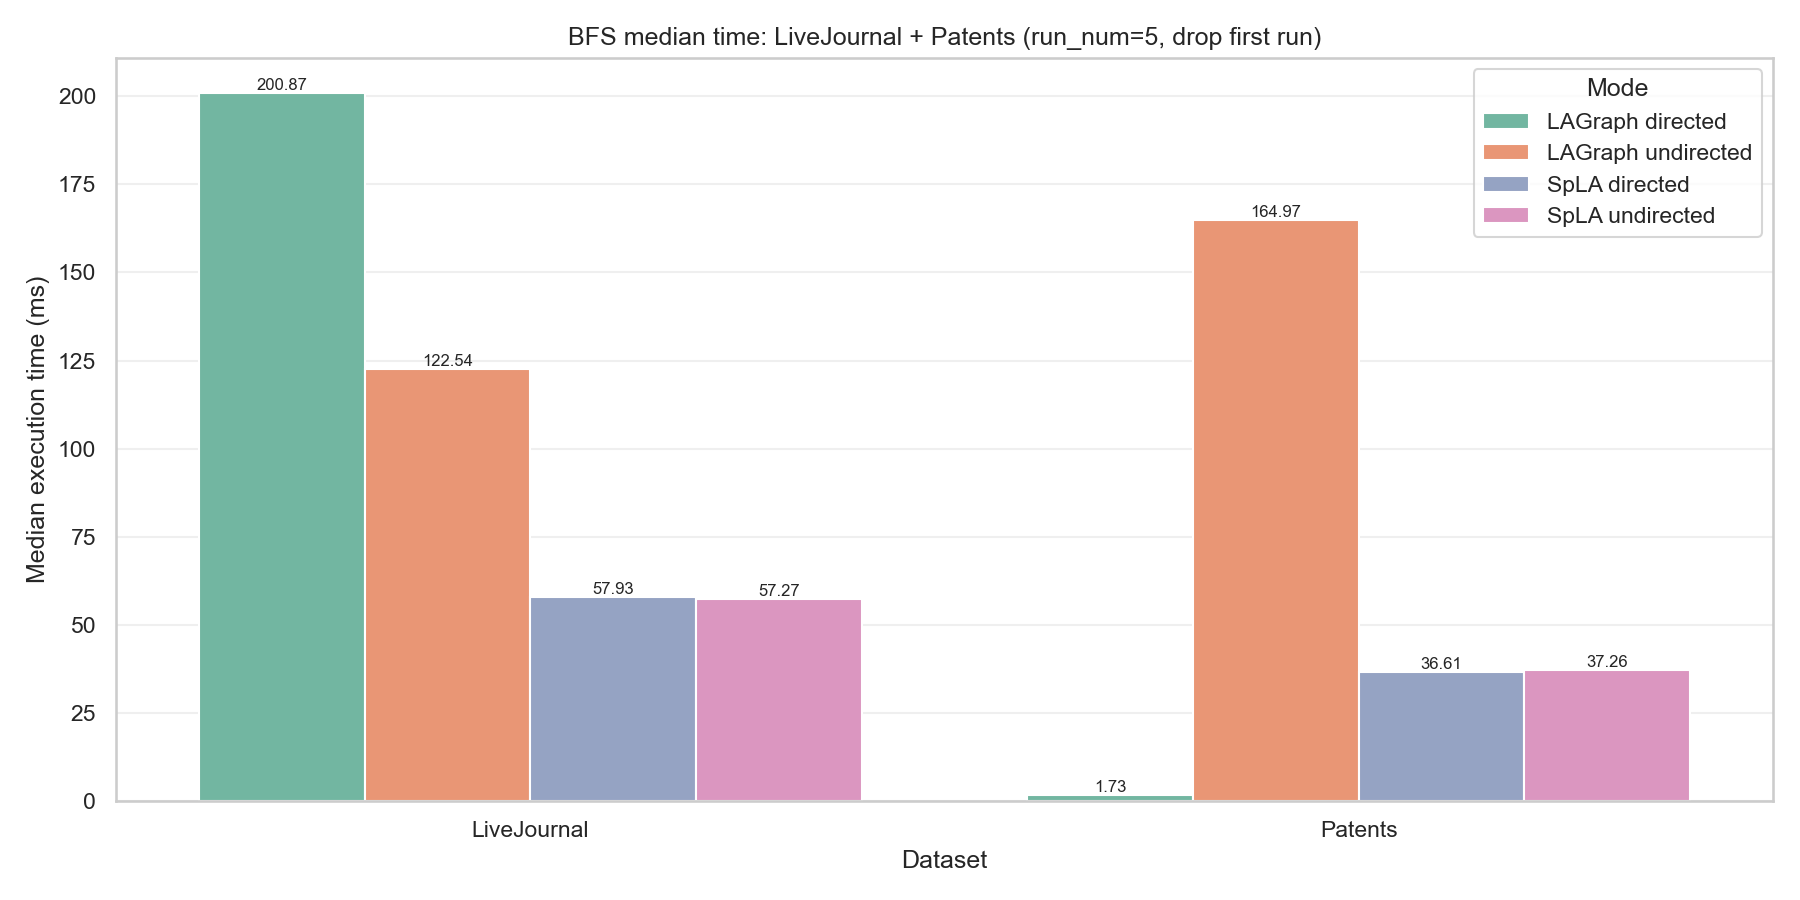
\includegraphics[width=1\textwidth]{pictures/bfs/bfs_modes_livejournal_patents_run5.png}
\end{frame}

\begin{frame}
	\frametitle{BFS}
	\begin{itemize}
		\item Push - обходит граф по направлению ребер.
		\item Pull - обходит граф против направления ребер.
		\item Алгоритм пытается проехать по улице с односторонним движением навстречу потоку. 
		\item Он найдет вершины, из которых можно прийти во фронт, а не те, в которые можно попасть из фронта.
		\item Чтобы алгоритм Direction-Optimizing BFS (переключение Push/Pull) корректно работал на направленных графах, для шага Pull необходимо использовать транспонированную матрицу.
	\end{itemize}

\end{frame}

\begin{frame}[fragile]
	\begin{minipage}{3in}
	  \begin{Verbatim}[fontsize=\scriptsize]
if (push || (push_pull && is_push_better)) \{
    exec_vxm_masked(frontier_new, v, frontier_prev, A, BAND_INT, BOR_INT, EQZERO_INT, zero, desc);
\} else \{
    exec_mxv_masked(frontier_new, v, A, frontier_prev, BAND_INT, BOR_INT, EQZERO_INT, zero, desc);
\}
	  \end{Verbatim}
	\end{minipage}
\end{frame}

\begin{frame}
  \frametitle{BFS}

	Выводы:

  \begin{itemize}
	\item Выполнение большого кол-ва итераций с маленьким фронтиром - отрицательно действует на производительность GPU
	\item Время обхода направленного графа зависит от его свойств - "длины" путей и "ширины" фронтиров. Высокий коэффициент кластеризации и малый диаметр соцсети позволяют быстро расширять фронтир и эффективно использовать параллелизм
	\item SPLA эффективнее на больших графах с большой компонентой связности. На малых графах или при высокой фрагментации LAGraph предпочтительнее из-за низкой задержки CPU
	\item SPLA с оптимизацией push-pull работает только на ненаправленных графах.
  \end{itemize}
\end{frame}

\begin{frame}
  \frametitle{SSSP}
  \begin{itemize}
    \item Исполнение алгоритма эффективнее на GPU 
    \item GPU лучше справляется с симметричными датасетами, в отличии от CPU    GPU (SPLA) покажет значительное преимущество на графах с плотной структурой и широким фронтиром
	\item SSSP в SPLA не работает с ориентированными графами 
  \end{itemize}

\end{frame}

\begin{frame}
  \frametitle{SSSP}

	\centering
	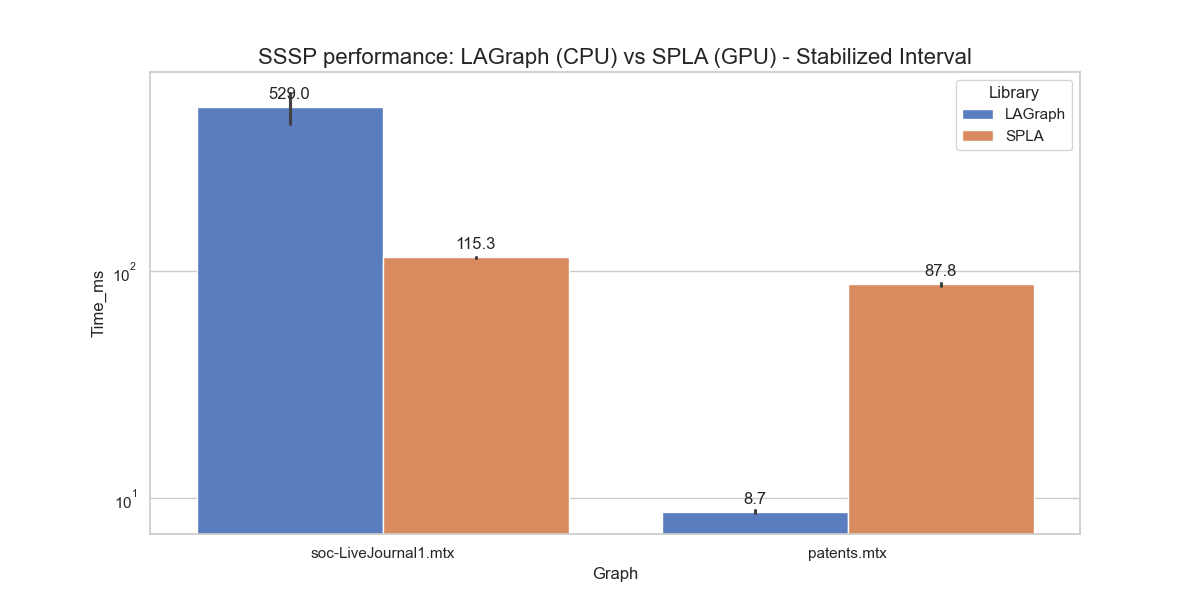
\includegraphics[width=1\textwidth]{pictures/sssp/mean_time.png}

\end{frame}

\begin{frame}
  \frametitle{SSSP}
	\centering
	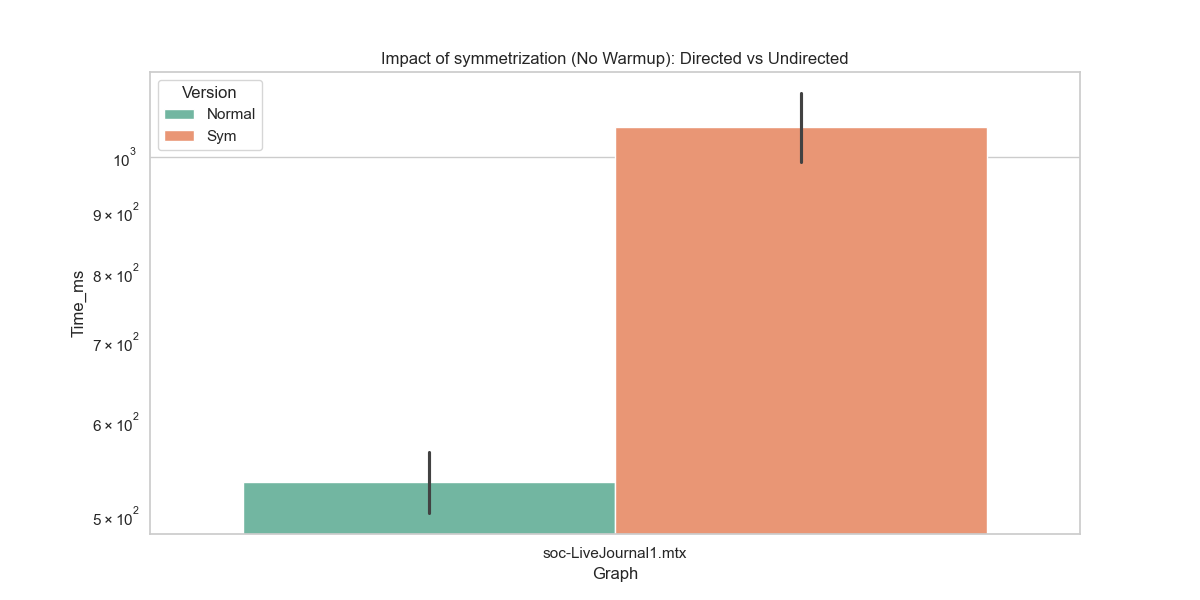
\includegraphics[width=1\textwidth]{pictures/sssp/mean_sym_time.png}

\end{frame}

\begin{frame}[fragile]
	\begin{minipage}{3in}
	  \begin{Verbatim}[fontsize=\scriptsize]
if (push || (push_pull && is_push_better)) \{
    exec_vxm_masked(frontier, dummy_mask, feedback, A, PLUS_FLOAT, MIN_FLOAT, ALWAYS_FLOAT, inf_init);
\} else \{
    exec_mxv_masked(frontier, dummy_mask, A, feedback, PLUS_FLOAT, MIN_FLOAT, ALWAYS_FLOAT, inf_init);
\}
	  \end{Verbatim}
	\end{minipage}
\end{frame}

\begin{frame}
  \frametitle{SSSP}
  \begin{itemize}
	  \item В графе патентов (где 3.7 млн узлов) вершина с наибольшим кол-вом исходящих ребер связана только с 776 другими вершинами. У LiveJournal вершина имеет в 20 раз больше выходящих ребер
	  \item На LiveJournal GPU работает в 4.7 раза быстрее CPU. Это "родная" среда для массивного параллелизма SPLA
	  \item Ситуация с поддержкой ориентированных графов - точно такая же, как и в BFS. (алгоритм использует hybrid push/pull execution) 

  \end{itemize}
	\textbf{Общий вывод:} Для алгоритма SSSP выбор вычислительного устройства критически зависит от топологии.

\end{frame}

\begin{frame}
  \frametitle{PageRank}
  \begin{itemize}
    \item Эффективность GPU-ускорения прямо пропорциональна регулярности структуры графа 
    \item  Низкая средняя степень узла делает использование GPU нецелесообразным    
	\item Неравномерность распределения в безмасштабных сетях снижает потенциал GPU по сравнению с регулярными структурами
  \end{itemize}
\end{frame}

\begin{frame}
  \frametitle{PageRank}
	\centering
	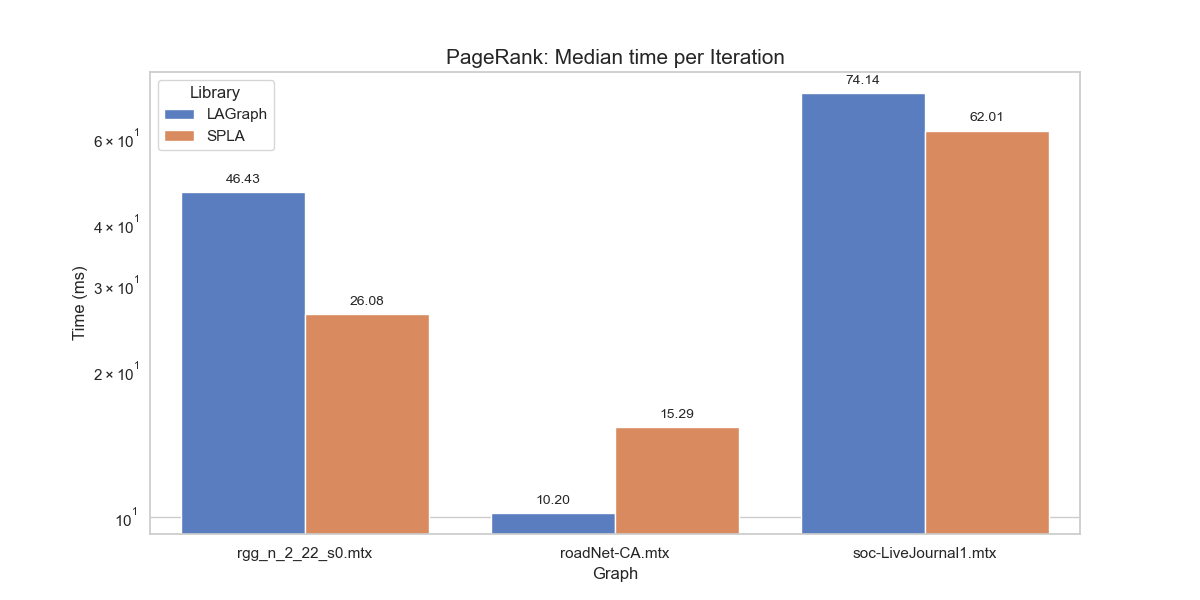
\includegraphics[width=1\textwidth]{pictures/pr/median_time.png}
\end{frame}

\begin{frame}
  \frametitle{PageRank}
	\centering
	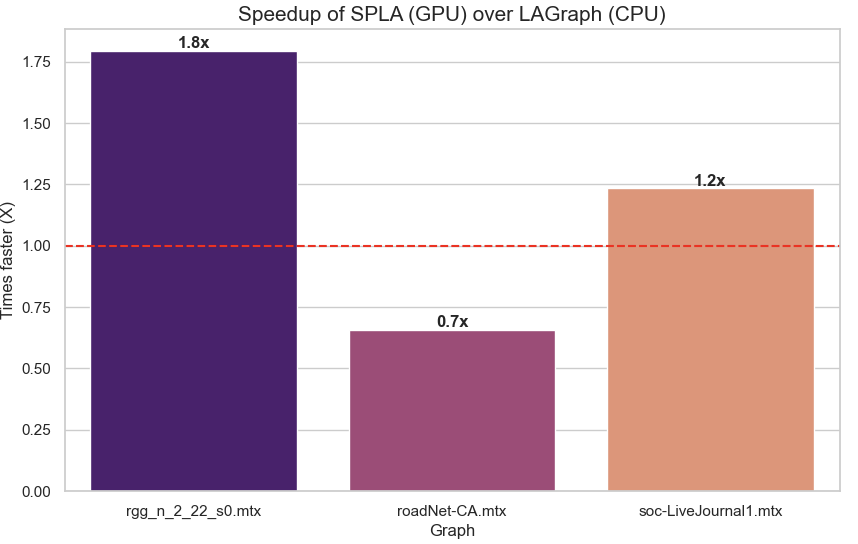
\includegraphics[width=1\textwidth]{pictures/pr/speedup.jpg}
\end{frame}

\begin{frame}
  \frametitle{PageRank}
	\centering
	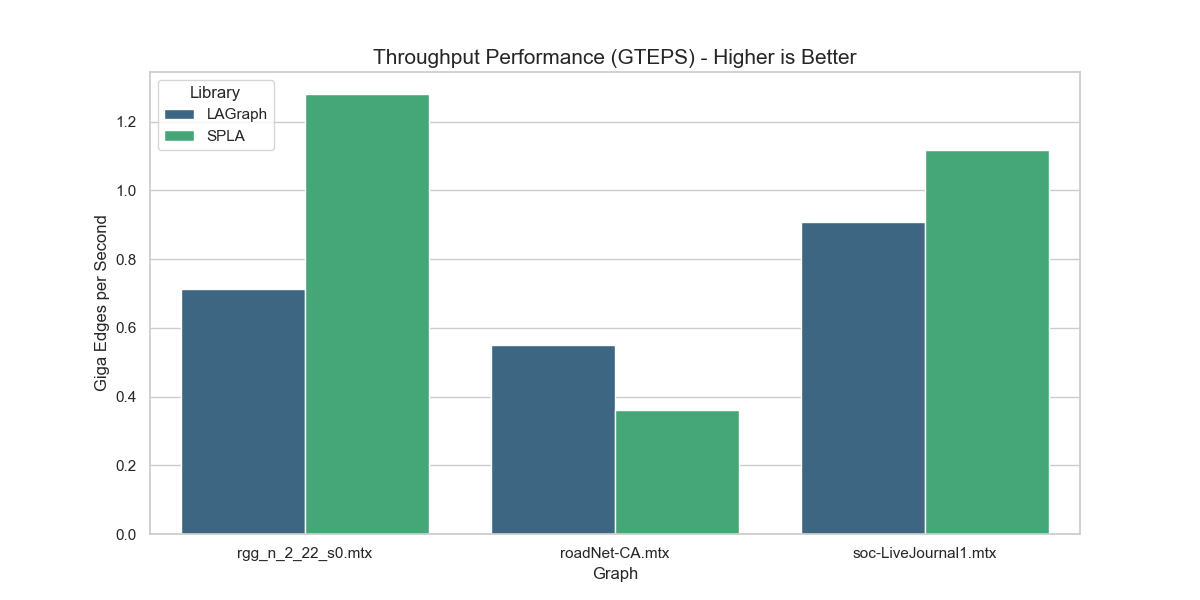
\includegraphics[width=1\textwidth]{pictures/pr/throughput.png}
\end{frame}

\begin{frame}
  \frametitle{PageRank}
	\begin{itemize}
		\item Cтепени узлов распределены равномерно, что минимизирует простой ядер GPU
		\item Дорожные графы эффективнее на CPU. Накладные расходы на запуск ядер и обращение к памяти GPU не окупаются малым объемом вычислений на одно ребро.

	\textbf{Общий вывод:} SPLA эффективен на "тяжелых" графах с большим количеством ребер, но его преимущество нивелируется при сильной разреженности (дороги) или экстремальной неравномерности (социальные сети).
	\end{itemize}

\end{frame}

\begin{frame}
  \frametitle{TC}
  \begin{itemize}
	  \item Архитектура GPU должна показывать многократное преимущество в данной задаче 
	  \item На разреженных графах с низкой средней степенью/ (road) эффективность GPU будет ниже, чем на плотных или регулярных из-за накаладных расходов    
		\item Для алгоритмов семейства Sandia на CPU предварительная сортировка узлов по степени критически важна для минимизации количества вычислений
  \end{itemize}
\end{frame}

\begin{frame}
  \frametitle{TC}
	\centering
	
\includegraphics[width=1\textwidth]{pictures/tc/mean_time.png}
\end{frame}

\begin{frame}
  \frametitle{TC}
	\centering
  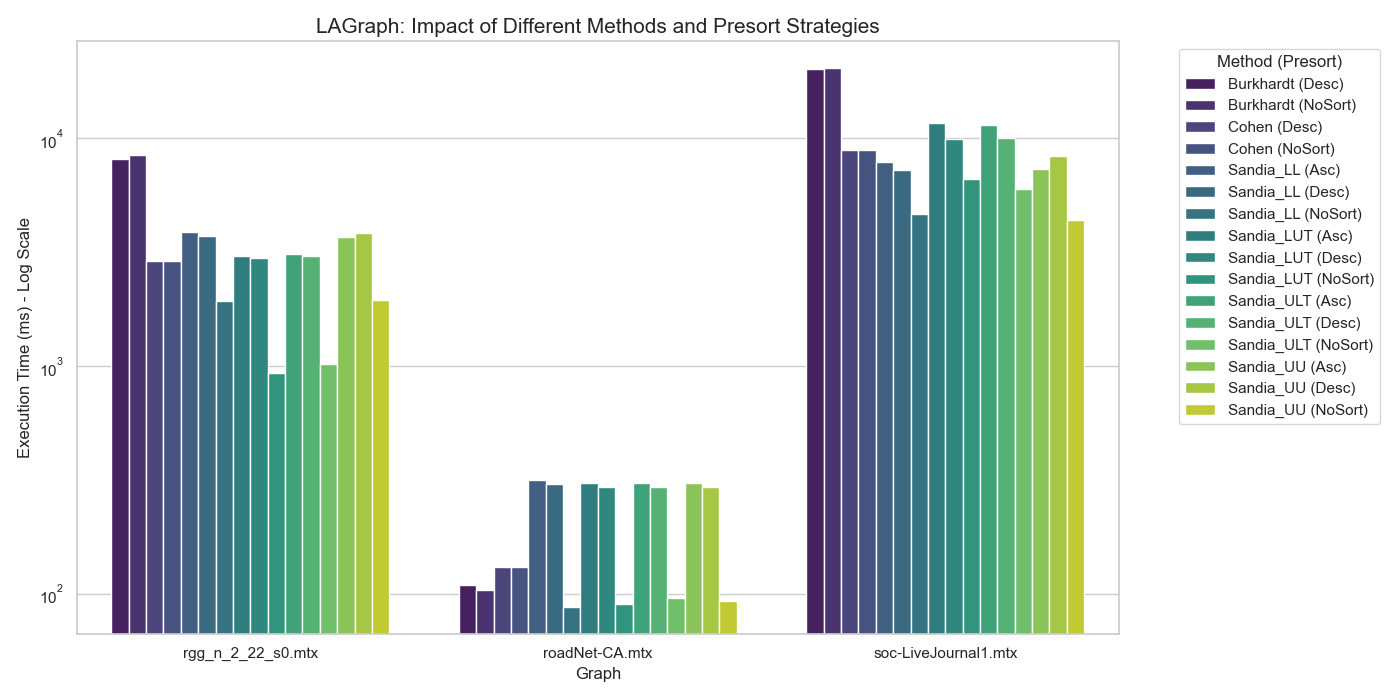
\includegraphics[width=1\textwidth]{pictures/tc/methods_time.png}
\end{frame}

\begin{frame}
  \frametitle{TC}
	\centering
  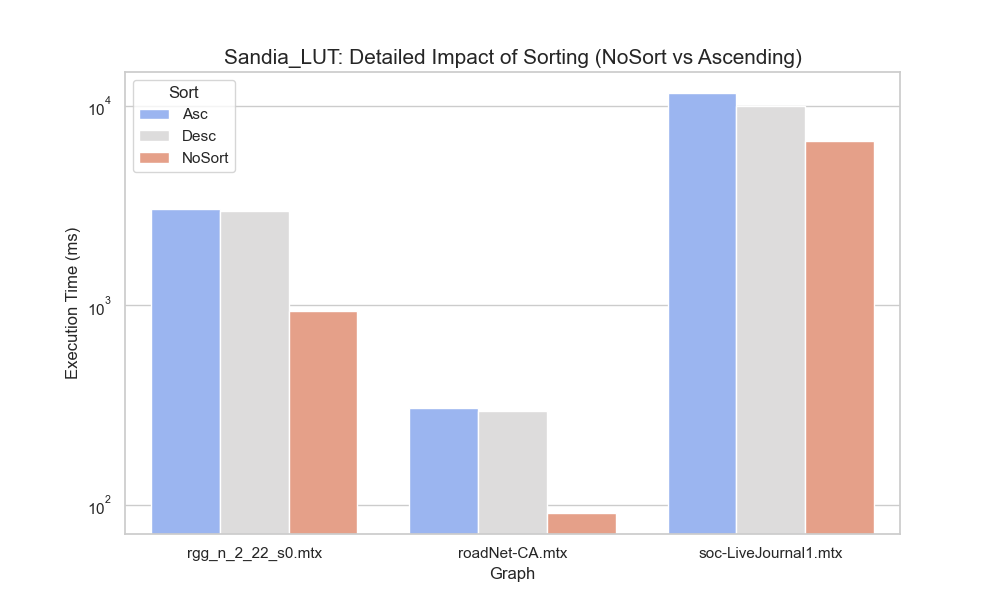
\includegraphics[width=1\textwidth]{pictures/tc/sandia_lut_methods_time.png}
\end{frame}

\begin{frame}
  \frametitle{TC}
	Основные операции в TC Sandia
  \begin{itemize}
	  \item Взять список сетей U
	  \item Взять список сетей V 
	  \item Найти пересечение 
  \end{itemize}
\end{frame}

\begin{frame}
  \frametitle{TC}
  Сортировка является ключевой оптимизацией в случае семейства алгоритмов Sandia. 
	Сортировка уменьшает стоимость одного пересечения увеличивая cache locality, меньше случайного доступа. 
	Условия включения сортировки при выбранном режиме AutoSort.
  \begin{itemize}
	  \item n > 2000
	  \item density > 10
	  \item mean > 3 * median (определяет насколько граф powel-law)
  \end{itemize}
\end{frame}

\begin{frame}
  \frametitle{TC}
	\begin{table}[htbp]
		\centering
\begin{tabular}{lcccc}
\hline
Name & Mean & Median & Ratio & Density \\
\hline
rgg\_n\_2\_22\_s0 & 14,4 & 14 & 1 & 14,47 \\
soc-LiveJournal1  & 14,2 & 4  & 3,5 & 14,12 \\
roadNet-CA        & 2,79 & 3  & 0,9 & 2,8 \\
\hline
\end{tabular}
		\caption{LAGraph TC, Graphs details}
		\label{tab:comparison}
	\end{table}
\end{frame}

\begin{frame}
  \frametitle{TC}
	\begin{itemize}
		\item На основе предыдущих графиков можем сделать вывод, что ни на одном графе (даже на soc-LiveJournal, который явно подходит под AutoSort) мы не получили прироста. 
		\item Наоборот, при выборе NoSort - производительность оказалась выше, чем при принудительно Asc и Desc.
		\item Причина падения производительности может заключаться в затратах на предварительную сортировку графа.
	\end{itemize}
\end{frame}
\begin{frame}[fragile]
	\begin{minipage}{3in}
	  \begin{Verbatim}[fontsize=\scriptsize]

//--------------------------------------------------------------------------
// sort the input matrix, if requested
//--------------------------------------------------------------------------

if (presort != LAGr_TriangleCount_NoSort)
\{
    // P = permutation that sorts the rows by their degree
    LG_TRY (LAGr_SortByDegree (&P, G, true,
        presort == LAGr_TriangleCount_Ascending, msg)) ;

    // T = A (P,P) and typecast to boolean
    GRB_TRY (GrB_Matrix_new (&T, GrB_BOOL, n, n)) ;
    GRB_TRY (GrB_extract (T, NULL, NULL, A, (GrB_Index *) P, n,
        (GrB_Index *) P, n, NULL)) ;
    A = T ;

    // free workspace
    LG_TRY (LAGraph_Free ((void **) &P, NULL)) ;
\}

	  \end{Verbatim}
	\end{minipage}
\end{frame}

\begin{frame}
  \frametitle{TC}
	\begin{table}[htbp]
	\centering
	\begin{tabular}{lccc}
	\hline
	Symbol & NoSort & Asc & Desc \\
	\hline
		mxm & 25,5\% (5,71s) & 22,9\% (5,72s) & 23,1\% (5,76s) \\
		Matrix\_extract & None & 9,4\% (2,36s) & 9,8\% (2,44s) \\
		Matrix\_reduce & 0,3\% (0,06s) & None & None \\
		SortByDegree & None & 1,4\% (0,36s) & 1,5\% (0,36s) \\
	\hline
	\end{tabular}
	\caption{LAGraph TC, sort variations}
	\label{tab:comparison}
	\end{table}
\end{frame}

\begin{frame}
  \frametitle{TC}

	После сортировки:
  \begin{itemize}
	  \item маленькие узлы пересекаются друг с другом (дёшево)
	\item хабы концентрируются и реже пересекаются с другими хабами
  \end{itemize}
\end{frame}

\begin{frame}
  \frametitle{TC}
  \begin{itemize}
	  \item Ускорение на GPU достигает 84.5х. Задача Triangle Counting, основанная на пересечении множеств, идеально ложится на архитектуру SPLA
	\item Предположение о том, что Ascending Sort всегда ускоряет TC на CPU, опровергнуто. Несмотря на схождение требований эвристик с характеристиками графа soc-LiveJournal1 - не получили прироста.
	\item Самой быстрой стратегией для TC на CPU является использование наиболее эффективного алгоритма (Sandia LUT или LL) на исходном порядке узлов (NoSort), чтобы избежать дорогостоящих операций перестановки матриц
	  \item Высокий GTEPS на дорогах говорит о том, что маскирование в SPLA работает исключительно эффективно даже при малом количестве треугольников  
  \end{itemize}
\end{frame}

%\addtocounter{framenumber}{1}
\appendix


\end{document}
